\chapter{Các khái Niệm Cơ Bản}
  \label{Chapter1} % For referencing the chapter elsewhere, use \ref{Chapter1} 
  \rhead{\bfseries Khóa Luận Tốt Nghiệp,Năm 2013}

  Để hiểu được tính chất vật lý của chất rắn mà cụ thể ở đây là chất bán dẫn việc tính  cấu trúc vùng năng lượng $\mathbf{E_n(k)}$ là hết sức quan trọng, và nó thể hiện hầu hết các tính chất điện và quang của vật liệu. Do tính chất tuần hoàn của mạng tinh thể, không gian xung lượng của hệ cũng có tính chất tuần hoàn, do đó cấu trúc vùng năng lượng chỉ cần xác định một khoãng hữu hạng k, và nếu như xét trong chất bán dẫn thì ta chỉ quan tâm một vài vùng ở cuối cùng bị lấp đầy, gọi là vùng hóa trị và một vài dải năng lượng đầu tiên còn trống gọi là vùng dẫn. Khi một vị trí trên vùng dẫn có electron thì ta có một hạt dẫn điện mang điện tích âm, khi một vị trí trên vùng cấm nó không có electrong nó tương đương với một hạt điện tích dương ở đó và được gọi là lỗ trống (hole), nó có ích khi ta tính các dòng. 
  Trong vật lý nguyên tử số hạng tương tác spin-orbit (SO) trong Hamiltonian được dẫn ra gần đúng từ phương trình Dirac [6] và đại lượng đó có giá trị sau
  \begin{equation}
  \mathcal{H}_{SO} = \frac{\hbar}{4m^2_0}\boldsymbol{\sigma} \cdot \left(\boldsymbol{\nabla} V_0\times \boldsymbol{p} \right) =  \frac{\hbar}{4m^2_0}\left(\boldsymbol{\sigma}\times \boldsymbol{\nabla}V_0\right)\cdot\boldsymbol{p}
  \end{equation}
  ở đây $\hbar$ là hằng số Planck, $m_0$ là khối lượng hiệu dụng của điện tử tự do, c là vận tốc ánh sáng, $\mathbf{p}$ là toán tử động lượng, $\mathbf{V}_0$ là thế Coulomb của nguyên tử và $\boldsymbol{\sigma} = \left(\sigma_x,\sigma_y,\sigma_z\right)$ là một véctơ ma trận Pauli và ta cũng biết rằng tương tác này làm thây đổi phổ năng lượng, làm tách spin.
  \section{Tương tác spin-orbit trong tinh thể chất rắn}
  Trong tinh thể chất rắn, phương trình chuyển động của điện tử có thể được miêu tả bởi cấu trúc vùng năng lượng $\mathbf{E}_n\left(\mathbf{k}\right)$, trong đó n là chỉ số đặc trưng(chỉ số vùng) cho giá trị khác nhau của $\mathbf{E}_n(\mathbf{k})$, ứng với mỗi giá trị của $\mathbf{k}$ (véctơ sóng), và ở đây số hạng tương tác SO cũng ảnh hưởng rất lớn đến cấu trúc vùng năng lượng  $\mathbf{E}_n\left(\mathbf{k}\right)$, ví dụ trong chất bán dẫn GaAs số hạng tương tác SO sẽ làm suy biến các mức năng lượng của spin up và spin down của tán sắc năng lượng, sự tách này là khá nhỏ cở một vài $meV$. Người ta đã ứng dụng hiệu ứng này vào việc tạo ra dòng photocurrent, tức là sinh ra dòng điện hoặc dòng spin trong chất bán dẫn bằng kích thích quang học thuần túy,trong mô hình 8$\times$8 kp có cả spin-orbit về mặt nguyên tắc là không suy biến và không thể viết 2 ma trận khối 4$\times$4.\\
  Tuy nhiên khi tính toán ta bỏ qua  một số hạng thứ 2 trong phương trình (4.4) thì mô hình trở thành suy biến, số hạng này được tham số hóa bởi tham số C trong mô hình Kane mở rộng, nếu tính đầy đủ thông số này nó sẽ gây ra một sự tách suy biến cở 0,1 $meV$ theo phương [110] nó là khá nhỏ có thể bỏ qua được nếu ta so sánh nó với mô hình kp 14$\times$14 tính đến cả tương tác vùng dẫn $p^*$ cho sự tách suy biến vào cỡ 1 $meV$ gần khe vùng. Từ mô hình kp 14$\times$14 ta có thể nhận lại mô hình kp 8$\times$8 nếu bỏ qua tương tác với vùng dẫn $p^*$ cụ thể là cho các thông số $P^{'}$, Q, và $\Delta^{-}$ trong phương trình (4.5) bằng 0.\\
  Các chất bán dẫn là tinh thể của các nguyên tử nhóm IV (Si,Ge) hay hợp chất của nhóm nguyên tử III và V(GaAs ,InSb) đặc điểm chung của chúng là lớp vỏ ngoài cùng không lắp đầy có thể là 3,4,5. điện tử phân bố trên 2 phân lớp s,p ví dụ: Si là ............... $3s^23p^2$ (nó chuyển thành$\dots 3s^13p^3$ khi liên kết các nguyên tử Si khác trong tinh thể ), như vậy khi một nguyên tử trong chất bán dẫn làm gì thì làm khi liên kết với nhau thì lớp vỏ ngoài của điện tử của nó được lắp đầy với 8 điện tử cụ thể là có 2 điện tử ở trạng thái s và 6 điện tử ở trạng thái p. Nhưng các trạng thái s và p không còn là trạng thái s và p của đơn nguyên tử  nữa \emph{mà là trạng thái s và p dùng chung của từng cặp nguyên tử}, hàm sóng mới là của trạng thái mới là tổ hợp tuyến tính (chồng chập) của hàm sóng điện tử của 2 nguyên tử, kết quả là 
  \begin{equation}
  \psi_+=\psi_1 +\psi_2  \qquad \psi_\_=\psi_1 -\psi_2
  \end{equation}
  chú ý ở trên ta viết một cách gần đúng lẽ ra phải có hằng số trước các hàm sóng $\psi_1$ và $\psi_2$ để cho dễ miêu tả (xem ở phụ lục), trong  đó $\psi_1,\psi_2$ là trạng thái điện tử của nguyên tử 1 và 2, trạng thái $\psi_+$ gọi là trạng thái liên kết(bonding) còn trạng thái $\psi_\_$ gọi là trạng thái phản liên kết(antiboding), dấu trừ hay dấu cộng là do hàm hám sóng $\psi_1,\psi_2$ có thể dương hay âm tùy ý vì chỉ có bình phương môđun hàm sóng mới có ý nghĩa vật lý.\\
  Biết hàm sóng thì ta có thể tính được năng lượng của trạng thái liên kết và phản liên kết, kết quả là từ 2 mức năng lượng s và p ta có 4 mức năng lượng sếp từ thắp đến cao s-boding,p-bonding và s-antibonding,p-antibonding, 2 mức thắp nhất là s-bonding, p-bonding lắp đầy với 8 điện tử. Cần chú ý rằng khi chuyển sang giải thích tinh thể bán dẫn thì ta chỉ quan tâm tới p-bonding có 6 trạng thái đã bị lấp đầy bởi 6 điện tử (nó sẽ chuyển thành vùng hóa trị suy biến 6 đã bị lấp đầy) và s-antibonding có 2 trạng thái trống, không có điện tử nào (nó sẽ chuyển thành vùng dẫn suy biến 2 còn trống). \emph{Tóm lại bây giờ chỉ còn 6 điện tử và 8 trạng thái chứ không phải 8 điện tử}.\\
  \begin{figure}[hc]
  \centering
  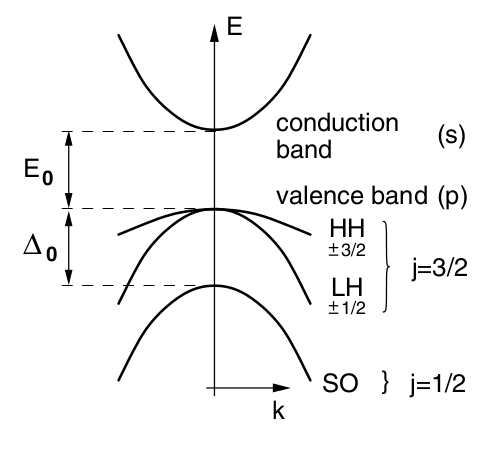
\includegraphics[width=0.50\textwidth]{./Figures/band1.png}
  %\rule{35em}{0.5pt}
  \caption[band structure]{Độ tách suy biến mức năng lượng do tương tác spin-orbit Ref [22]}
  \label{fig:band structure}
  \end{figure}
  Do tương tác của spin-orbit, các trạng thái ứng với $j=1/2$ bị tách suy biến có mức năng lượng thắp hơn năng lượng của trạng thái $j=3/2$, vùng năng lượng ứng với $j=1/2$ gọi là vùng hóa trị SO đôi khi người ta gọi nó là (split-off valence band)[15]. Vùng này suy biến bậc 2 theo hình chiếu của $j$ lênh trục $\mathbf{z}$ là $m_j=\pm 1/2$, vùng hóa trị ứng với $j=3/2$ gồm có 4 trạng thái ứng với các hình chiếu của $j$ lên trục $\mathbf{z}$ là $ m_j=\pm 3/2,\pm 1/2$, trong đó trạng thái ứng với $m_j=\pm 3/2$ là suy biến có cùng mức năng lượng và còn gọi là vùng lỗ trống nặng (heavy-hole) và $m_j = \pm 1/2$ là suy biến có cùng mức năng lượng và còn gọi là vùng lỗ trống nhẹ (light-hole), chú ý nếu như trong bán dẫn khối vùng lỗ trống nhẹ và lỗ trống nặng trùng nhau nên có suy biến bậc bốn.
  \section{Tương tác trao đổi}
  Tương tác trao đổi là kết quả của tương tác tĩnh điện Coulomb giữa những điện tử, do hàm sóng mô tả một cặp điện tử là hàm phản xứng nên nếu spin của hai điện tử là song song, phần tọa độ của hàm sóng phải là phản đối xứng:$\psi_{\uparrow\uparrow}\left(\mathbf{r}_1,\mathbf{r}_2\right)=-\psi_{\uparrow\uparrow}\left(\mathbf{r}_2,\mathbf{r}_1\right)$. Trường hợp ngược lại nếu spin của 2 điện tử là phản song song thì phần tọa độ của hàm sóng phải là đối xứng $\psi_{\uparrow\downarrow}\left(\mathbf{r}_1,\mathbf{r}_2\right)=-\psi_{\uparrow\downarrow}\left(\mathbf{r}_2,\mathbf{r}_1\right)$. vì vậy khả năng để 2 điện tử đến trong trường hợp sau là lớn hơn so vớ trường hợp trước, so với những điện tử có spin phản song thì spin điện tử song song cách xa hơn do đó lực đẩy giữa chúng là nhỏ hơn cũng như tương tác trao đổi tĩnh điện nhỏ hơn.\\
  Trong chất bán dẫn tương tác trao đổi thường không đóng góp lớn, ngoại trừ đối với những chất bán dẫn từ (CdMnTe) và mặt phân giới bán dẫn. 
  \section{Tương tác hyperfine với spin của hạt nhân}
  Đây là tương tác từ giữa spin của hạt nhân với spin của điện tử, tương tác này sẽ quan trọng nếu mang hạt hạt nhân trong chất bán dẫn có spin khác không như GaAs. Nếu hạt nhân này phân cực tương tác này tương đương với một từ trường hiệu dụng của hạt nhân tác dụng lên spin của điện tử. Trong GaAs khi $100\%$ hạt nhân phân cực từ trường này có giá trị hiệu dụng vài Tesla. Cũng như tương tác spin-orbit tương tác hyperfine tăng mạnh trong những nguyên tử có Z lớn, ngoài ra còn có tương tác từ đây là tương tác giữa mômen của một cặp điện tử, tương tác này rất yếu nó thường không được xét trong chất bán dẫn.
 


  \section{Lý thuyết nhóm trong vật lý}
  \subsection{Định nghĩa nhóm}
  Một tập hơp $\mathcal{G} =\{ a,b,c\ldots \}$ được gọi là một nhóm nếu nó tồn tại một phép nhân nhóm thỏa mản các tiên đề sau:
  \begin{enumerate}
  \item[1/] a,b $\in$ $\mathcal{G}$;\qquad\qquad c=a.b$\in \mathcal{G}$ \qquad\qquad\qquad\qquad(\emph{tính đóng})
  \item[2/] a,b,c $\in \mathcal{G}$;\qquad (ab).c=a.(b.c) \qquad\qquad\qquad\qquad (\emph{tính kết hợp})
  \item[3/]$\exists e \in\mathcal{G};\qquad g.e=e.g=g \qquad\forall g\in\mathcal{G}$ \  \qquad\qquad(\emph{phần tử đợn vị e duy nhất})
  \item[4/]$\forall a\in \mathcal{G} \qquad \exists b\in\mathcal{G}$;\qquad a.b=e ie, b=$a^{-1}$\qquad\qquad (\emph{phần tử nghịch đảo})
  \end{enumerate}
  \subsection{Nhóm điểm}
  $1/$ \textbf{Nhóm trực giao} $\mathcal{O}(3)$ \textbf{trong không gian 3 chiều}:
  \begin{equation}
  \mathcal{O}(3) = \{\mathcal{O}=\mathcal{O}_{ij}:\mathcal{O}_{ij}\in\mathcal{R},1\leq i,j\leq 3 ,\mathcal{O}^T\mathcal{O}=\mathbb{E}_3\}
  \end{equation}
  trong đó $\mathbb{E}_3$ là ma trận đơn vị, ta có thể chứng minh $det(\mathcal{O})=\pm1$,và nhóm $\mathcal{SO}(3)$ là nhóm con bất biến thậm chí là chuẩn tắc, các phần tử của nó là các phép quay trong không gian 3 chiều còn các phần tử của lớp kề nó là phép quay kèm theo một phép đối xứng gương [21]
  \begin{equation}
  \mathcal{SO}(3) = \{\mathcal{O}\in\mathcal{O}(3):det(\mathcal{O})=1\}
  \end{equation}
  Ý nghĩa hình học của nhóm $\mathcal{SO}(3)$: Ta có thể chứng minh nếu $\mathcal{O}\in\mathcal{SO}(3)$ thì tồn tại một véctơ $\vec{f}$ sao cho:
  \begin{equation}
  \mathcal{O}\vec{f}=1.\vec{f} \qquad |\vec{f}|=1
  \end{equation}
  ta chọn hệ trực chuẩn $\mathbf{f}_1,\mathbf{f}_2,\mathbf{f}_3$, hệ trực chuẩn ở đây có ý nghĩa là $\langle \mathbf{f}_i,\mathbf{f}_j\rangle=\delta_{ij}$, ta sẽ tìm dạng ma trận $\mathcal{O}$ trong cơ sở này, để tìm nó ta giải hệ phương trình sau:
  \begin{equation}
  \begin{cases} 
  \mathcal{O}\mathbf{f}_1 &=\alpha_1\mathbf{f}_1 +\beta_1\mathbf{f}_2 +\gamma_1\mathbf{f}_3 \\
   \mathcal{O}\mathbf{f}_2 &=\alpha_2\mathbf{f}_1 +\beta_2\mathbf{f}_2 +\gamma_2\mathbf{f}_3  \\
   \mathcal{O}\mathbf{f}_3 &=\alpha_3\mathbf{f}_1 +\beta_3\mathbf{f}_2 +\gamma_3\mathbf{f}_3 
   \end{cases} 
   \end{equation}
  giải hệ phương trình trên ta có kết qủa của ma trận $\mathcal{O}$ như sau:
  \begin{equation}
  \mathcal{O}=\mathcal{C}_3(\alpha)=\begin{pmatrix}
  \cos\alpha &-sin\alpha & 0\\
  \sin\alpha &\cos\alpha &0\\
  0 &0 &1
  \end{pmatrix}
  \end{equation}
  %-----------------------------Hinh coordinte-------------------------

  \begin{figure}[hc]
  \centering
  \ifx\du\undefined
    \newlength{\du}
  \fi
  \setlength{\du}{15\unitlength}
  \begin{tikzpicture}
  \pgftransformxscale{1.000000}
  \pgftransformyscale{-1.000000}
  \definecolor{dialinecolor}{rgb}{0.000000, 0.000000, 0.000000}
  \pgfsetstrokecolor{dialinecolor}
  \definecolor{dialinecolor}{rgb}{1.000000, 1.000000, 1.000000}
  \pgfsetfillcolor{dialinecolor}
  \pgfsetlinewidth{0.100000\du}
  \pgfsetdash{}{0pt}
  \pgfsetdash{}{0pt}
  \pgfsetbuttcap
  {
  \definecolor{dialinecolor}{rgb}{0.000000, 0.000000, 0.000000}
  \pgfsetfillcolor{dialinecolor}
  % was here!!!
  \pgfsetarrowsend{latex}
  \definecolor{dialinecolor}{rgb}{0.000000, 0.000000, 0.000000}
  \pgfsetstrokecolor{dialinecolor}
  \draw (22.900000\du,12.950000\du)--(30.900000\du,12.950000\du);
  }
  \pgfsetlinewidth{0.100000\du}
  \pgfsetdash{}{0pt}
  \pgfsetdash{}{0pt}
  \pgfsetbuttcap
  {
  \definecolor{dialinecolor}{rgb}{0.000000, 0.000000, 0.000000}
  \pgfsetfillcolor{dialinecolor}
  % was here!!!
  \pgfsetarrowsend{latex}
  \definecolor{dialinecolor}{rgb}{0.000000, 0.000000, 0.000000}
  \pgfsetstrokecolor{dialinecolor}
  \draw (22.900000\du,12.950000\du)--(22.950000\du,5.300000\du);
  }
  \pgfsetlinewidth{0.100000\du}
  \pgfsetdash{}{0pt}
  \pgfsetdash{}{0pt}
  \pgfsetbuttcap
  {
  \definecolor{dialinecolor}{rgb}{0.000000, 0.000000, 0.000000}
  \pgfsetfillcolor{dialinecolor}
  % was here!!!
  \pgfsetarrowsend{latex}
  \definecolor{dialinecolor}{rgb}{0.000000, 0.000000, 0.000000}
  \pgfsetstrokecolor{dialinecolor}
  \draw (22.850000\du,12.900000\du)--(16.450000\du,16.600000\du);
  }
  \pgfsetlinewidth{0.050000\du}
  \pgfsetdash{}{0pt}
  \pgfsetdash{}{0pt}
  \pgfsetmiterjoin
  \pgfsetbuttcap
  {
  \definecolor{dialinecolor}{rgb}{0.000000, 0.000000, 0.000000}
  \pgfsetfillcolor{dialinecolor}
  % was here!!!
  \pgfsetarrowsend{latex}
  \definecolor{dialinecolor}{rgb}{0.000000, 0.000000, 0.000000}
  \pgfsetstrokecolor{dialinecolor}
  \pgfpathmoveto{\pgfpoint{21.150000\du}{8.650000\du}}
  \pgfpathcurveto{\pgfpoint{23.350000\du}{9.650000\du}}{\pgfpoint{27.250000\du}{8.600000\du}}{\pgfpoint{23.700000\du}{7.250000\du}}
  \pgfusepath{stroke}
  }
  % setfont left to latex
  \definecolor{dialinecolor}{rgb}{0.000000, 0.000000, 0.000000}
  \pgfsetstrokecolor{dialinecolor}
  \node[anchor=west] at (22.800000\du,4.400000\du){$\mathbf{f_3}$};
  % setfont left to latex
  \definecolor{dialinecolor}{rgb}{0.000000, 0.000000, 0.000000}
  \pgfsetstrokecolor{dialinecolor}
  \node[anchor=west] at (16.900000\du,17.300000\du){$\mathbf{f_1}$};
  % setfont left to latex
  \definecolor{dialinecolor}{rgb}{0.000000, 0.000000, 0.000000}
  \pgfsetstrokecolor{dialinecolor}
  \node[anchor=west] at (30.200000\du,13.950000\du){$\mathbf{f_2}$};
  % setfont left to latex
  \definecolor{dialinecolor}{rgb}{0.000000, 0.000000, 0.000000}
  \pgfsetstrokecolor{dialinecolor}
  \node[anchor=west] at (22.850000\du,13.700000\du){O};
  \end{tikzpicture}
  \caption[phép quay trục $f_3$]{Phép quay quanh trục$\mathbf{f_3}$ }
  \label{fig:phép quay trục $f_3$}
  \end{figure}

  như vậy ma trận $\mathcal{O}$ chính là ma trận của phép quay quanh trục $\mathbf{f}_3$ một góc $\theta$, quay theo quy tắc bàn tay phải,làm tương tự cho các trục quay $\mathbf{f}_1,\mathbf{f}_2$ ta có kết quả sau:
  \begin{equation}
  \mathcal{O}=\mathcal{C}_2(\beta)=\begin{pmatrix}
  \cos\beta &0 &sin\beta\\
  0 &1 & 0\\
  -\sin\beta &0 &\cos\beta
  \end{pmatrix}
  \end{equation}
  \begin{equation}
  \mathcal{O}=\mathcal{C}_2(\gamma)=\begin{pmatrix}
  1 &0 &0 \\
  0 &\cos\gamma &-\sin\gamma\\
  0 &\sin\gamma &\cos\gamma
  \end{pmatrix}
  \end{equation}
  Thông thường các hệ số 1,2,3 được thây bởi $\mathit{x,y,z}$ trong khi ta thực hành trên các bài toán vật lý, xét nhóm quay trong không gian ba chiều $\mathcal{SO}(3)$. Mọi phép quay không gian ba chiều quanh gốc tọa độ $\mathbf{O}$ đều có thể được thực hiện dưới dạng tổ hợp của ba phép quay liên tiếp sau đây: phép quay góc $\alpha$ quanh trục $\mathbf{O}\mathit{z}$ chuyển các trục tọa độ $\mathbf{O}\mathit{x}$ và $\mathbf{O}\mathit{y}$ thành $\mathbf{O}\mathit{x}^{'}$ và $\mathbf{O}\mathit{y}^{'}$, 
  phép quay góc $\beta$ quanh trục mới $\mathbf{O}\mathit{y}^{'}$ chuyển
  các trục mới $\mathbf{O}\mathit{z}$ và $\mathbf{O}\mathit{x}$ thành $\mathbf{O}\mathit{z}^{'}$ và $\mathbb{O}\mathit{x}^{''}$, phép quay góc $\gamma$ quanh trục mới $\mathbf{O}\mathit{z}^{'}$ (xem hình 2.11). Ba thông
  số $\alpha,\beta,\gamma$ gọi là ba góc Euler và . Ký hiệu phép quay với ba góc Euler $\mathfrak{D}(\alpha,\beta,\gamma)$\\
  \begin{enumerate}
  \item[1.] Thực hiện phép quay 1 góc $\alpha$ quanh trục $\mathcal{O}z\qquad\sum\longrightarrow\sum^{'},0\leq \alpha\leq 2\pi$ 
  \item[2.] Thực hiện phép quay 1 góc $\beta$ quanh trục $\mathcal{O}y^{'}\qquad\sum^{'}\longrightarrow\sum^{''},0\leq \alpha\leq \pi$ 
  \item[3.] Thực hiện phép quay 1 góc $\gamma$ quanh trục $\mathcal{O}z^{'}\qquad\sum^{''}\longrightarrow\sum^{'''},0\leq \gamma\leq 2\pi$ 
  \end{enumerate}

  \begin{figure}[hc]
  \centering
  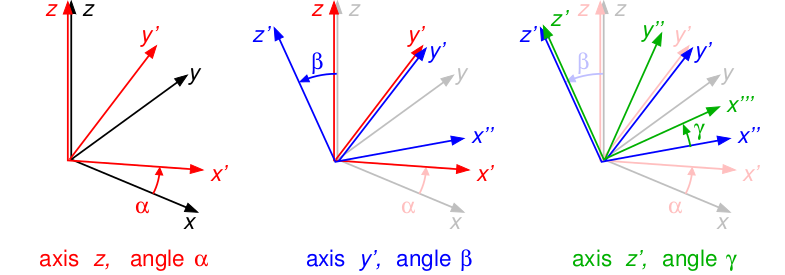
\includegraphics[width=0.70\textwidth]{./Figures/Selection_001.png}
  %\rule{35em}{0.5pt}
  \caption[phép quay]{Phép quay quanh trục$\mathcal{O}z,\mathcal{O}y^{'},\mathcal{O}z^{'}$ }
  \label{fig:phép quay}
  \end{figure}
  \begin{align}
  \mathfrak{D}(\alpha,\beta,\gamma)&=
  \mathfrak{D}_z(\alpha)\mathfrak{D}_y(\beta)\mathfrak{D}_z(\gamma)\notag\\
  &=\begin{pmatrix}
  \cos\alpha &-sin\alpha & 0\\
  \sin\alpha &\cos\alpha &0\\
  0 &0 &1
  \end{pmatrix}
  \begin{pmatrix}
  \cos\beta &0 &sin\beta\\
  0 &1 & 0\\
  -\sin\beta &0 &\cos\beta
  \end{pmatrix}
  \begin{pmatrix}
  \cos\alpha &-sin\alpha & 0\\
  \sin\alpha &\cos\alpha &0\\
  0 &0 &1
  \end{pmatrix}\\
  &=\begin{pmatrix}
  \cos\alpha\cos\beta\cos\gamma -\sin\alpha\sin\gamma & \cos\alpha\cos\beta\sin\gamma +\sin\alpha\sin\gamma & -\cos\alpha\sin\beta \\
  -\sin\alpha\cos\beta\cos\gamma -\cos\alpha\sin\gamma & -\sin\alpha\cos\beta\sin\gamma +\cos\alpha\sin\gamma &\sin\alpha\sin\beta \\
  \sin\beta\cos\gamma &\sin\beta\sin\gamma & \cos\beta \notag
  \end{pmatrix}
  \end{align}
  \section{Phép quay trong cơ học lượng tử}
  \textbf{1.Toán tử của phép quay:} Với bất kỳ phép quay trong hệ vật lý chúng ta có thể biểu diễn mối liên hệ giữa toán tử phép quay $\mathfrak{D}(R)$ và trạng thái của hệ vật lý sau khi thực hiện phép quay như sau:
  \begin{equation}
  \vert \Psi\rangle_{R} = \mathfrak{D}(R) \vert \Psi\rangle_{R}
  \end{equation}  
  ta sẽ dẫn ra dạng toán tử phép quay $\mathfrak{D}(R)$,gọi $\mathfrak{D}(\mathbf{n},d\phi)$ là toán tử của phép quay quanh hệ một góc $d\phi$ vô cùng bé quanh một trục có véctơ đơn vị là $\mathbf{n}$, trong phép quay này tọa độ của hạt trong hệ biến đổi như sau:
  \begin{equation}
  \mathbf{r_i} \longrightarrow \mathbf{r}_i^{'} = \mathbf{r_i} +d\mathbf{r_i} \qquad i=1,2,\dots, N
  \end{equation} 
  trong đó $d\phi = d\phi\left(n\times r_i\right)$, khai triển hàm sóng $\vert \Psi\rangle$ quanh điểm $d\mathbf{r}_i$  và chỉ lại số hạng bậc nhất sau vài phép biến đổi ta có dạng toán tử $\mathfrak{D}(\mathbf{n},d\phi)$ như sau:
  \begin{equation}
  \mathfrak{D}(\mathbf{n},d\phi) = 1 -i\left(\frac{\mathcal{J}\mathbf{n}}{\hbar}\right)d\phi
  \end{equation}
  ở đây ta sẽ định nghĩa đại lượng $\mathcal{J}$ là toán tử mômen động lượng toàn phần và $\mathcal{J}$ cũng gọi là một vi tử của phép quay quanh hệ một góc vô cùng bé \\
  Bây giờ ta xét hệ quay quanh 1 góc hữu hạn $\phi$ quanh trục $\mathbf{n}$ gọi $\mathfrak{D}(\mathbf{n},d\phi)$  là toán tử của phép quay này ta có:
  \begin{equation}
  \mathfrak{D}(\mathbf{n},\phi + d\phi) =\mathfrak{D}(\mathbf{n},d\phi)\mathfrak{D}(\mathbf{n},\phi)
  \end{equation}
  hoặc ta có thể biểu diễn dưới dạng sau:
  \begin{equation}
  \mathfrak{D}(\mathbf{n},d\phi) = \lim_{N\longrightarrow\infty}\left(1 -i\frac{\mathcal{J}\mathbf{n}}{\hbar}\frac{\phi}{N}\right)^N = exp\left(-i\phi\frac{\mathbf{n}\mathcal{J}}{\hbar}\right)
  \end{equation}
  \begin{figure}[hc]
  \centering
  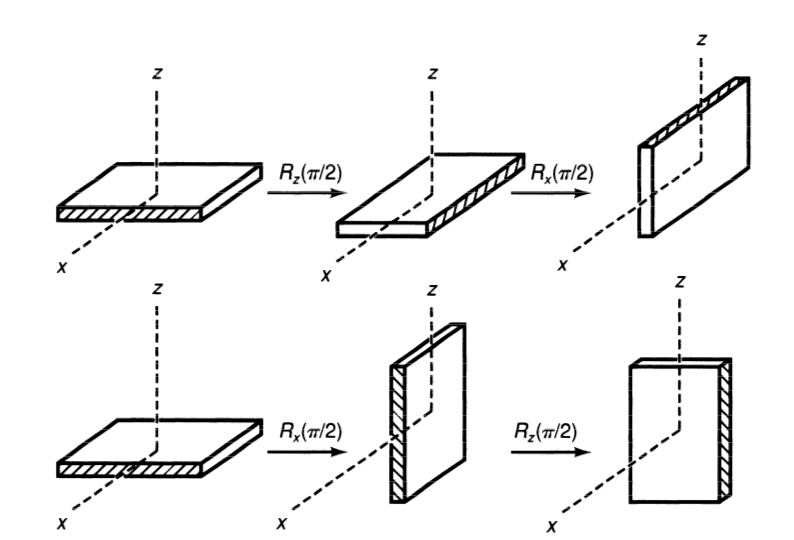
\includegraphics[width=0.70\textwidth]{./Figures/rota.png}
  %\rule{35em}{0.5pt}
  \caption[sự không giao hoán của phép quay]{Thí dụ minh họa sự không giao hoán của phép\\ quay quanh các trục của phép quay Ref [9] }
  \label{fig:sự không giao hoán của phép quay}
  \end{figure}\\
 Công thức (2.15) cho ta thấy các toán tử $\mathcal{J}_x,\mathcal{J}_y,\mathcal{J}_z$ là không giao hoán với nhau.\\
  \textbf{2.Phép quay là một nhóm:} Do đó nó đầy đủ tính chất nhóm tức tính đóng, tính kết hợp, tồn tại phần tử đơn vị và phần tử nghịch đảo. Một tập hợp các phép quay của toán tử của $\mathfrak{D}(R)$ cũng là một nhóm, xét 2 phép quay $\mathfrak{D}_1$,$\mathfrak{D}_2$ ta có thể tính nó như thế nào, dựa vào biểu thức (2.15) ta dễ dàng suy ra được tích $\mathfrak{D}_1 .\mathfrak{D}_2$ như sau:
  \begin{equation}
  \mathfrak{D}(R_2)\mathfrak{D}(R_1)=\mathfrak{D}(R_2 R_1)
  \end{equation} 
  sử dụng (2.14) khai triển nó tới số hạng $d\phi^2$ đồng thời sử dụng công thức sau [9]
  \begin{equation}
  \mathfrak{D}_x(\varepsilon)\mathfrak{D}_y(\varepsilon) -\mathfrak{D}_y(\varepsilon)\mathfrak{D}_x(\varepsilon) =\mathfrak{D}_z(\varepsilon^2)- \mathfrak{D}_{any}(0)
  \end{equation}
  ta dễ dàng có được điều này:
  \begin{equation}
  \left[ \mathcal{J}_i,\mathcal{J}_j\right] = i\hbar\varepsilon_{ijk}\mathcal{J}_k
  \end{equation}
  trong đó $\varepsilon_{ijk}$ là tenxo phản đối xứng được định nghĩa như sau. Gọi p là số hoán đưa (i,j,k) về tập hợp (1,2,3) khi đó:
  \begin{equation}
  \varepsilon_{ijk}=\begin{cases}
  &+1 \qquad \text{nếu} i\neq j\neq k \qquad \text{và p là số chẳn}\\
  &-1 \qquad \text{nếu} i\neq j\neq k \qquad \text{ và nếu p là số lẻ}\\
  & 0 \qquad \text{nếu có từ 2 chỉ số trở lên trùng nhau }
  \end{cases}
  \end{equation}
  \textbf{3.Hàm riêng và trị riêng của mômen động lượng toàn phần:} Dựa vào định nghĩa (2.19)  ta có thể tìm được trị riêng của $\mathcal{J}^2$ và $\mathcal{J}_z$  mà không cần phải biết dạng tường minh của 2 toán tử này, với mục đích đó ta đưa vào các toán tử thang $\mathcal{J}_{\pm}$ như sau:
  \begin{equation}
  \mathcal{J}_{\pm} =\mathcal{J}_x \pm \mathcal{J}_y 
  \end{equation}
  tác dụng toán tử $\mathcal{J}_{\pm}$ lên trạn thái $\vert j,m\rangle$ sau vài phép biến đổi ta có
  \begin{equation}
  \mathcal{J}_{\pm}\vert j,m\rangle = \sqrt{(j\mp m)(j\pm m+1)}\hbar\vert j,m\pm 1\rangle
  \end{equation}
  để cho biểu thức ket bên vế phải chuẩn hóa. ta cần phải giới hạn giá trị của m là (2$j$ +1)
  \begin{equation}
   m= -j,-j+1,\dots ,j-1,j
  \end{equation} 
  như vậy chỉ với lập luận dựa trên hệ thức giao hoán  và tính tự liên hợp của mômen động lượng ta đi đến những kết luận quan trọng sau đây:
  \begin{enumerate}
  \item[1.] Bình phương mômen động lượng bị lượng tử hóa theo quy tắc  $\mathcal{J}^2 = j(j+1)\hbar^2$, trong đó số lượng tử $j$ chỉ nhận những giá trị $j=0,1/2,1,3/2,2,5/2,\dots$
  \item[2.] Với $j$ cho trước tồn tại (2$j$+1) trạng thái $\vert j,m\rangle$ chú ý nó cũng là số chiều trong biễu diễn bất khả quy, và số lượng m được cho bởi công thức (2.32), hình chiếu mômen động lượng trên trục $z$ bị lượng tử hóa theo quy tắc $\mathcal{J}_z=m\hbar$. Ngoài ra còn có dạng ma trận của toán tử mômen động lượng, phép cộng mômen động lượng và hàm sóng của hạt có chứa spin $\dots$ thêm khảo thêm [3,9].
  \end{enumerate}
  \section{Lý thuyết nhiễu loạn giả suy biến}
  \textbf{Lý thuyết nhiễu loạn giả suy biến:} Đó là một phương pháp rất tổng quát và hữu ích để chúng ta tính toán gần đúng các thành phần không chéo hóa của Hamiltonian độc lập với thời gian, nhưng nó cũng có thể dùng cho nhiều trường hợp khác trong cơ học lượng tử, phương pháp này đôi khi người ta gọi là phương pháp L$\ddot{o}$wdin partitioning nội dung của phương pháp này như sau [10,11,22,23,24]:
  Thành phần Hamiltonian ta có thể tách ra hai thành phần, một thành phần $\mathcal{H}_0$ như ta đã biết là thành phần không nhiễu loạn có trị riêng năng lượng là $E_n$ và hàm riêng là $\vert \psi_n\rangle$, $\mathcal{H}^{'}$ là thành phần nhiễu loạn có thể xem số hạng $\mathbf{kp}$ trong phương trình (4.1) do đó ta có thể viết Hamiltonian như sau:
  \begin{equation}
  \mathcal{H} =\mathcal{H}_0 +\mathcal{H}^{'}
  \end{equation}
  Giả sử chúng ta có thể chia hàm riêng $\vert\psi_n\rangle$ ra làm 2 thành phần, một tập hợp thành phần lớp $\mathcal{A}$ và một tập hợp thành phần lớp $\mathcal{B}$, sao cho ta chỉ xét các thành phần tập hợp lớp $\mathcal{A}$ còn $\mathcal{B}$ ta có thể  bỏ qua chú ý ta chỉ bỏ qua $\mathcal{B}$ thôi còn các hiệu ứng giửa tập hợp $\mathcal{A}$ và $\mathcal{B}$ thì ta không bỏ qua, tức là các thành phần thuộc lớp $\mathcal{A}$ ta chọn như sau, bao gồm 2 lỗ trống nặng, 2 lỗ trống nhẹ và 2 spin-off band, còn tập hợp $\mathcal{B}$ là các thành phần còn lại.
  Lý thuyết nhiễu loạn giả suy biến xây dựng cơ bản dựa trên ý tưởng là toán tử Unitary $e^{-S}$ như vậy ta có thể thu được một Hamiltonians mới nhờ phép biến đổi sau:
  \begin{equation}
  \tilde{\mathcal{H}} =e^{-S}\mathcal{H}e^{S}
  \end{equation}
  trong thành phần ma trận $\langle\psi_m\vert \tilde{\mathcal{H}} \vert \psi_l\rangle$ khi ta xét đến số hạng nhiễu loạn $\mathcal{H}^{'}$ thì thành phần $\langle\psi_m\vert \mathcal{H}^{'} \vert \psi_l\rangle$ của tập hợp $\mathcal{B}$ sẽ triệt tiêu nếu ta xét trong các dãy  2 lỗ trống nặng, 2 lỗ trống nhẹ và 2 spin-off band, chúng ta có thể miêu tả loại bỏ các thành phần không chéo hóa trong $\mathcal{H}$ như hình vẽ dưới đây:
  \begin{figure}[hc]
  \centering
  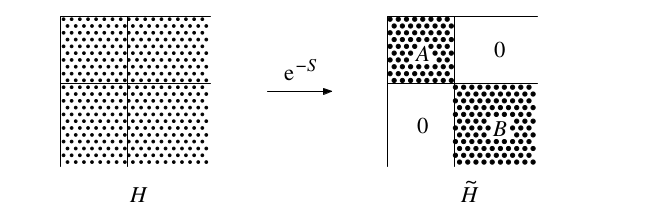
\includegraphics[width=0.70\textwidth]{./Figures/lowd.png}
  %\rule{35em}{0.5pt}
  \caption[Removal of off-diagonal elements of H]{Hamiltonian được đưa về dạng chéo hóa khối nhờ toán tử S,\\ gồm 2 thành phần $\mathcal{A},\mathcal{B}$ Ref[22]}
  \label{fig:Removal of off-diagonal elements of H}
  \end{figure}
  \begin{figure}[hc]
  \centering
  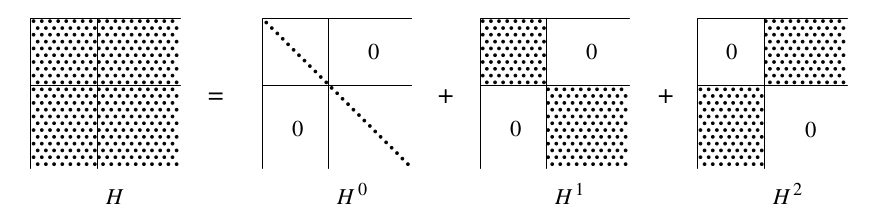
\includegraphics[width=0.70\textwidth]{./Figures/lowd2.png}
  %\rule{35em}{0.5pt}
  \caption[ Representation of H ]{Trình bày $\mathcal{H}$ thông qua các Hamiltionian $\mathcal{H}^0 + \mathcal{H}^1 +\mathcal{H}^2$ Ref[22]}
  \label{fig: Representation of H }
  \end{figure}
  Đại lượng S trong biểu thức (2.24) có nhiệm vụ biến đổi $\mathcal{H}^2$ về dạng tương tự như $\mathcal{H}^1$ trong khi vẫn giữ được hình thức chéo hóa khối của thành phần $\mathcal{H}^0+\mathcal{H}^1$ , để xác định đước toán tử S ta cần khai triển S dưới dạng chuổi Taylor như sau:
  \begin{equation}
  e^S = 1 +S + \frac{1}{2!}S^2 +\frac{1}{3!}S^3 +\dotsi
  \end{equation}
  và thây biểu thức này vào (2.24) ta có, chú ý rằng toán tử S là phản Hermitian tức $S^{\dagger} =-S$, ví dụ phép biến đổi từ biễu diễn Schr$\ddot{o}$dinger sang biễu diễn Heisenberg thì đại lượng S có giá trị là $\frac{i}{\hbar}Ht$
  \begin{equation}
  \tilde{\mathcal{H}} = \sum_{j=0}^{\infty}\frac{1}{j!}[\mathcal{H},S]^{j} = \sum_{j=0}^{\infty}\frac{1}{j!}[\mathcal{H}^0 +\mathcal{H}^1,S]^{j}+\sum_{j=0}^{\infty}\frac{1}{j!}[\mathcal{H}^2,S]^{j}
  \end{equation}
  ở đây giao hoán tử $\mathcal{A},\mathcal{B}$ được định nghĩa như sau:
  \begin{equation}
  [\mathcal{A},\mathcal{B}]^{j} = [\cdots\underbrace{[\mathcal{A},\mathcal{B}],\mathcal{B},\cdots \mathcal{B}}_{j\longrightarrow \infty}
  \end{equation}
  vì S làm cho thành phần không chéo hóa khối của $\mathcal{H}^2$ nên thành phần khối chéo hóa $\mathcal{H}_d$ có trong $\tilde{\mathcal{H}}$ gồm có $[\mathcal{H}^0 +\mathcal{H}^1,S]^{j}$ với j là chẵn còn sồ hạng $[\mathcal{H}^2,S]^{j}$ ới j là lẻ:
  \begin{equation}
  \tilde{\mathcal{H}}_d  = \sum_{j=0}^{\infty}\frac{1}{(2j)!}[\mathcal{H}^0 +\mathcal{H}^1,S]^{(2j)}+\sum_{j=0}^{\infty}\frac{1}{(2j+1)!}[\mathcal{H}^2,S]^{(2j+1)}
  \end{equation}
  ngược lại thành phần khối không chéo hóa $\mathcal{H}_n$ có trong $\mathcal{H}$ gồ có $[\mathcal{H}^0 +\mathcal{H}^1,S]^{j}$ với j là lẻ còn số hạng $[\mathcal{H}^2,S]^{j}$ với j là chẳn:
   \begin{equation}
  \tilde{\mathcal{H}}_n  = \sum_{j=0}^{\infty}\frac{1}{(2j+1)!}[\mathcal{H}^0 +\mathcal{H}^1,S]^{(2j+1)}+\sum_{j=0}^{\infty}\frac{1}{(2j)!}[\mathcal{H}^2,S]^{(2j)}
  \end{equation}
  vì theo đầu bài ta đã nói toán tử S được định nghĩa làm cho các thành phần khối không chéo hóa $\mathcal{H}_n =0$ là bằng không, ta chọn S tới số hạng bậc 3
  \begin{equation}
  S =S^{(1)} +S^{(2)} +S^{(3)} +\cdots
  \end{equation}  
  sử dụng biểu thức (2.31) kết hợp với $\mathcal{H}_n =0$ ta có kết quả sau:
  \begin{align}
  [\mathcal{H}^0,S^{(1)}] &= -\mathcal{H}^2 \notag\\
  [\mathcal{H}^0,S^{(2)}] &= -[\mathcal{H}^1,S^{(1)}] \notag\\
  [\mathcal{H}^0,S^{(3)}] &= -[\mathcal{H}^1,S^{(2)}] -\frac{1}{3}[[\mathcal{H}^2,S^{(1)}],S^{(2)}] \notag\\
  \cdots &= \cdots
  \end{align}
  giải phương trình (2.32) cho ta giá trị S cần tìm,gợi ý nhân 2 vế với két-véctơ và bra-véctơ $\vert nk\rangle$ và vì $\mathcal{H}^2$ ta có:
   \begin{align}
   S_{ml}^{(1)} &=-\frac{\mathcal{H}_{ml}^{'}}{E_m -E_l} \notag\\
   S_{ml}^{(2)}&= \frac{1}{E_m -E_l}\left[\sum_{m^{'}}\frac{\mathcal{H}_{mm^{'}}-\mathcal{H}_{m^{'}l}}{E_m^{'} -E_l}- \sum_{l^{'}}\frac{\mathcal{H}_{ml^{'}}-\mathcal{H}_{l^{'}l}}{E_m -E_{l^{'}}} \right]\notag\\
   S_{ml}^{(1)} &=\frac{1}{E_m -E_l}\notag\\
   &\times \biggl[-\sum_{m^{'},m^{''}}\frac{\mathcal{H}_{mm^{''}}\mathcal{H}_{m^{''}m}\mathcal{H}_{m^{'}l}}{(E_{m^{''}}-E_{l})(E_{m^{'}}-E_l)} 
  -\sum_{l^{'},l^{''}}\frac{\mathcal{H}_{ml^{'}}\mathcal{H}_{l^{'}l^{''}}\mathcal{H}_{l^{''}l}}{(E_{m^{'}}-E_{l^{''}})(E_{m}-E_l^{'})} \notag\\
  &+\sum_{l^{'},m^{'}}\frac{\mathcal{H}_{mm^{'}}\mathcal{H}_{m^{'}l^{'}}\mathcal{H}_{l^{'}l}}{(E_{m^{'}}-E_{l})(E_{m^{'}}-E_l^{'})} 
  +\sum_{l^{'},m^{'}}\frac{\mathcal{H}_{mm^{'}}\mathcal{H}_{m^{'}l^{'}}\mathcal{H}_{m^{'}l}}{(E_{m}-E_{l^{'}})(E_{m^{'}}-E_l^{'})}\notag\\
  &+\frac{1}{3}\sum_{l^{'},m^{'}}\frac{\mathcal{H}_{ml^{'}}\mathcal{H}_{l^{'}m^{'}}\mathcal{H}_{m^{'}l}}{(E_{m^{'}}-E_{l})(E_{m^{'}}-E_l^{'})} 
  +\frac{1}{3}\sum_{l^{'},m^{'}}\frac{\mathcal{H}_{ml^{'}}\mathcal{H}_{l^{'}m^{'}}\mathcal{H}_{m^{'}l^{'}}}{(E_{m}-E_{l^{'}})(E_{m^{'}}-E_l^{'})}\notag\\
  &+\frac{2}{3}\sum_{l^{'}m^{'}}\frac{\mathcal{H}_{ml^{'}}\mathcal{H}_{l^{'}m^{'}}\mathcal{H}_{m^{'}l}}{(E_{m^{'}}-E_{l})(E_{m^{'}}-E_l^{'})} \biggr]\notag \\
  &\cdots = \cdots
   \end{align}
  ở đây chỉ số $m,m^{'},m^{''}$ tương ứng với các trạng thái thuộc nhóm $\mathcal{A}$ còn các chỉ số $l,l^{'},l^{''}$ tương ứng với các trạng thái thuộc tập hợp $\mathcal{B}$  và $\mathcal{H}_{ml}\equiv \langle \psi_m \vert \mathcal{H} \vert\psi_l\rangle$, thây biểu thức (2.33) vào trong (2.29) ta tìm được dạng Hamiltonians chéo hóa khối cần tìm:
  \begin{equation}
  \tilde{\mathcal{H}} = \mathcal{H}^{(0)}+\mathcal{H}^{(1)}+H^{(2)}+\mathcal{H}^{(3)}+\mathcal{H}^{(4)}+\cdots
  \end{equation} 
  các thành phần Hamiltonians được trình bày ở mục (4.3). Ở đây tôi muốn nhấn mạnh rằng các mẫu số năng lượng ở mục (4.3) trong phương trình (4.11) rút ra từ trạng thái của nhóm $\mathcal{A}$ và trạng thái của nhóm $\mathcal{B}$. Trạng thái nhóm  $\mathcal{A}$ và nhóm $\mathcal{B}$ được chọn sao cho năng lượng của chúng là tách rời nhau, vì vậy ta có thể sử dụng các phương trình ở (4.11) cho các trạng thái của nhóm $\mathcal{A}$ chứa các thành phần tùy ý (có thể chưa biết), hoặc biết một cách chính xác, ngoài ra có một vài kỹ thuật được trình bày về vấn đề nhiễu loạn suy biến bạn có thể tham khảo ở đây\protect\footnote{In [9], Sakurai presents a three-level system (problem 5.12, p. 348)}, để phân tích nó ta dùng phần mềm Maple\protect\footnote{Maple is a registered trademark of Waterloo Maple Inc.}
  \section{Gần đúng Hatree-Fock}
  Để giải phương trình chuyển động của các toán tử $\chi_{k_{\parallel}}^{\lambda\lambda^{'}}=\langle a_{\lambda k_{\parallel}}^{\dagger}a_{\lambda^{'} k_{\parallel}}\rangle$ trong phương trình (5.16) thì ta cần phải ngắt chuỗi của nó, vì trong phương trình của nó ta thấy ứng với hai toán tử bên vế trái thì bên vế phải lại có bốn toán tử $\dots$ cứ như thế lặp đi lặp lại ta sẽ không giải được do đó ta cần phải sử dụng một phương pháp gần đúng, ở đây tôi sử dụng phương pháp gần đúng Hatree-Fock [1,15,17,18], xét phương trình chỉ có chứa hai toán tử có dạng sau đây:
  \begin{align}
  \frac{d}{dt}\langle \mathcal{AB}\rangle &= \frac{d}{dt}\langle \mathcal{AB}\rangle_{HF} +\left( \frac{d}{dt}\langle \mathcal{AB}\rangle - \frac{d}{dt}\langle \mathcal{AB}\rangle_{HF}\right)\notag\\
  &=\frac{d}{dt}\langle \mathcal{AB}\rangle_{HF} +\frac{d}{dt}\langle \mathcal{AB}\rangle_{col}
  \end{align}
  trong đó số hạng $\langle \mathcal{AB}\rangle_{HF}$ là số hạng đóng góp Hatree-Fock trong phương trình chuyển động, trong khi số hạng $\langle \mathcal{AB}\rangle_{col}$ là nhứng đóng góp số hạng bậc cao trong phương trình chuyển động trong trường hợp này là bốn toán tử, đôi khi ta gọi nó là số hạng mô tả va chạm hoặc tán xạ được tính gần đúng trong thời gian khử pha $T_2$ [2], còn đại lượng
  $\langle \mathcal{AB}\rangle_{col}=\chi_{k_{\parallel}}^{\lambda\lambda^{'}}/T_2$ sẽ là đại lượng cần phải tính trong phương trình triển khai (5.16). 
  \begin{figure}[hc]
  \centering
  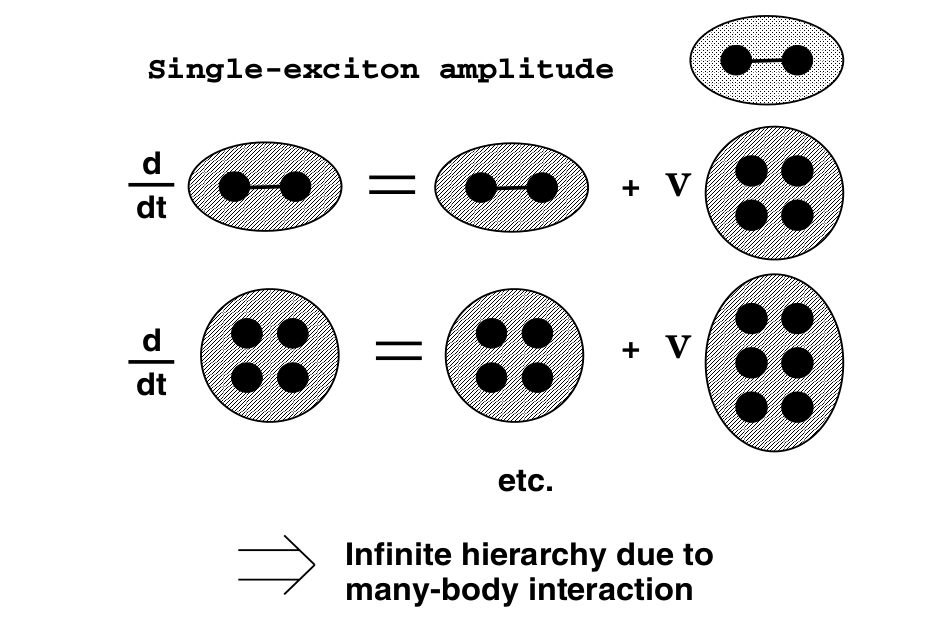
\includegraphics[width=0.70\textwidth]{./Figures/hatree-fock.png}
  %\rule{35em}{0.5pt}
  \caption[Hatree-Fock]{Phương trình chuyển động hữu hạn của hàm phân cực trong chất bán dẫn}
  \label{fig:Hatree-Fock}
  \end{figure}
  \begin{figure}[hc]
  \centering
  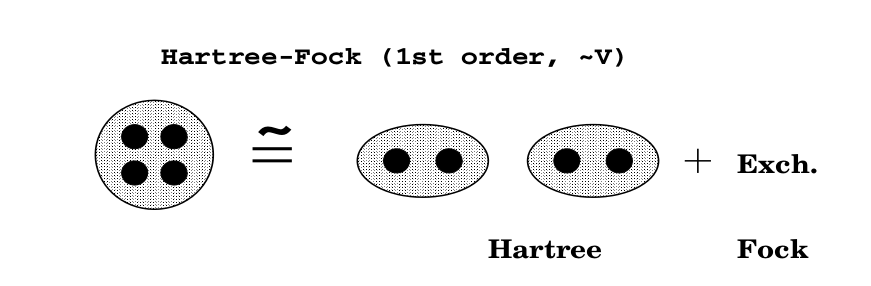
\includegraphics[width=0.70\textwidth]{./Figures/hatree-fock1.png}
  %\rule{35em}{0.5pt}
  \caption[Hatree-Fock]{Phương trình chuyển động được tính trong gần đúng Hatree-Fock Ref[19]}
  \label{fig:Hatree-Fock}
  \end{figure}
 Xét một ví dụ 
  \begin{align}
  \langle a_{k+q}^{\dagger}b_{-k}a_{k^{'}}a_{k+q}\rangle = \langle a_{k^{'}+q}^{\dagger}a_{k+q}\rangle\langle b_{-k}a_{k^{'}}\rangle - \langle a_{k^{'}+q}^{\dagger}a_{k^{'}}\rangle\langle b_{-k}a_{k+q}\rangle
  \end{align}
  và bây giờ ta giả sử $a_{k}^{\dagger}\propto e^{i\omega_k t}$ và $a_{k^{'}}\propto e^{-i\omega_{k^{'}} t}$ và ta có:
  \begin{equation}
  \langle a_{k}^{\dagger}a_{k^{'}}\rangle \propto e^{i(\omega_k -\omega_{k^{'}})}
  \end{equation}
  nó được biết đến như là phương pháp gần đúng pha ngẫu nhiên (Random Phase Approximation [1,15], ý tưởng gần đúng này cho rằng giá trị trung bình của các cặp toán tử $\langle a_{k}^{\dagger}a_{k^{'}}\rangle$ có sự phụ thuộc theo phase và thời gian như trên. Khi ta lấy tổng theo $k$ trị trung bình này thì chỉ có các số hạng chứa $k = k^{'}$ được giử lại, còn các số hạng khác do phase khác không nên bị dao động và trung bình theo thời gian đóng góp khác bằng không, với những lập luận ta viết lại biểu thức (2.36) như sau:
  \begin{align}
  \langle a_{k+q}^{\dagger}b_{-k}a_{k^{'}}a_{k+q}\rangle &= \langle a_{k^{'}+q}^{\dagger}a_{k+q}\rangle\langle b_{-k}a_{k^{'}}\rangle\delta_{kk^{'}} - \langle a_{k^{'}+q}^{\dagger}a_{k^{'}}\rangle\langle b_{-k}a_{k+q}\rangle\delta_{q,0}\notag \\
  &=n_{ek+q}p_k\delta_{k,k^{'}} - n_{ek^{'}}p_{k}\delta_{q,0}
  \end{align} 
  số hạng thứ 2 trong phương trình kia bị loại bỏ vì ta không xét trường hợp q=0
